\documentclass[a4paper]{article}

\usepackage{fancyhdr}
\usepackage[left=1.375in,right=1.375in]{geometry}
\usepackage[dvips]{graphicx}
\usepackage{color}
\usepackage{url}
\usepackage{natbib}
\usepackage{listings}
\usepackage{amssymb}
\usepackage{amsmath}

\definecolor{CodeBackground}{rgb}{0.9, 0.95, 0.95}
\lstset{ %
    %language=Python,
    %alsolanguage=hoc,
	backgroundcolor=\color{CodeBackground},
	frame=single,  % the zero-width frame is to make
	framerule=0pt, % the colour extend beyond the listing
	basicstyle=\ttfamily,
	%xleftmargin=2em,
	%xrightmargin=2em
}
\lstdefinestyle{display}{
  basicstyle=\ttfamily\footnotesize,
}

\lstdefinestyle{numberlines}{
  basicstyle=\ttfamily\footnotesize,
  numbers=left,
  stepnumber=1
}


\definecolor{INCFBlue}{rgb}{0.0,0.59,1.0}

\newcommand\nmlClass[1]{{\tt #1}}


\begin{document}

\pagestyle{empty}


\begin{center}
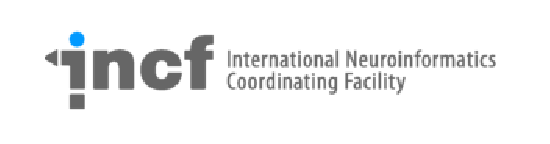
\includegraphics[width=0.7\columnwidth]{images/incf.eps}
\end{center}

\vspace*{1cm}

\noindent\rule{\columnwidth}{1pt}
\noindent\rule{\columnwidth}{2pt}

\vspace*{1cm}

\begin{center}

\noindent{\Huge \bf Specification Document:}\\

\vspace{0.5cm}
\noindent{\Large \bf Network Interchange format for NEuroscience (NineML): \\ Abstraction Layer}\\
\vspace{0.5cm}
\noindent{\large INCF Task Force on Multi-Scale Modeling}\\
\vspace{0.5cm}

\noindent{\large Version: 0.1}\\

\end{center}

\vspace*{0.75cm}

\noindent\rule{\columnwidth}{2pt}
\noindent\rule{\columnwidth}{1pt}

\vspace*{3cm}
\noindent{\Large

\begin{center}
{\bf Authors (in alphabetical order): }
\end{center}

\noindent Hugo Cornelis, Andrew Davison, Mikael Djurfeldt, Sean Hill, Eilif Muller, Ivan Raikov \\

%\vspace*{0.5cm}

\noindent {\bf Date:} \today

}


\title{NineML Specification Document}

\newpage
\pagestyle{plain}

\tableofcontents

\section{Introduction}

With an increasing number of studies related to large-scale neuronal
network modeling, the International Neuroinformatics Coordinating
Facility (INCF) has identified a need for standards and guidelines to
ease model sharing and facilitate the replication of results across
different simulators. To create such standards, the INCF has formed a
program on Multiscale Modeling to develop a common standardized
description language for neuronal network models.

The name of the proposed standard is NineML (Network Interchange for
Neuroscience Modeling Language) and its first version is aimed at
descriptions of large networks of spiking neurons.

\subsection{Scope}

The purpose of NineML is to provide a computer language for
succinct and unambiguous description of computational neuroscience models of
networks of spiking neurons.

NineML is intended to describe the network architecture, parameters
and equations that govern the dynamics of a network of spiking
neurons. The behavioral aspects of such a system, such as input
stimulus, and the numerical implementation details, such as
integration method used, have to be described using different
techniques.  Model description in NineML is intended to be formal in
the sense that it is possible to interpret it unambiguously.

\subsection{Objective}

The key concepts of spiking neuron network modeling are:

\begin{enumerate}
\item spiking neurons
\item synapses
\begin{enumerate}
\item Post-synaptic membrane current mechanisms
\item Short-term synaptic dynamics (a la Markram et. al. 1998)
\item Long-term synaptic modifications (STDP, learning, etc.)
\end{enumerate}
\item populations of neurons
\item connectivity patterns across populations of neurons.
\end{enumerate}

Accordingly, NineML defines a set of mathematical abstractions that
are capable of representing these concepts.

\subsection{Design Considerations}


\subsubsection{User layer and Abstraction layer}

The design of NineML is divided into two semantic layers: an abstraction
layer (the subject of the present document) that provides the core
concepts, mathematics and syntax with which model variables and state
update rules are explicitly described, and a user layer that provides a
syntax to specify the instantiation and parameterization of a network
model in biological terms.

As the User Layer provides the mechanism for instantiating and
parameterization of the model elements that have been defined in the
Abstraction Layer, it is clearly essential that these two layers share
a complementary and compatible design philosophy. There must be a
clear definition of which aspects of a model are defined in the User
Layer and which are defined in the Abstraction Layer. In addition, the
mechanisms and syntax for naming and addressing Abstraction Layer definitions
is ideally re-used in the User Layer to keep things simple for the user.

\subsubsection{Implementation assumptions}

One of the goals identified by task force members, was to maintain a
clear distinction between the role of NineML and a simulator. NineML
should provide only the information necessary for any given simulator
to instantiate the network models in a simulator agnostic way.  For
example, NineML should specify the neuron membrane equation to solve,
but not how to solve it.  In addition, for implementation and
performance reasons, it is important to keep the language layer
“close” to the simulator – such that the language layer is not
responsible for maintaining separate representations of the
instantiated network.

\subsubsection{Language syntax}

It is envisioned that the language should not require a
specific syntax or rely on any given technology or platform.
Rather it is anticipated that the language can be
employed by defining the model elements in a variety of different
syntaxes including a native (domain specific) language, Python, Java,
and XML (for example).


\section{Abstraction Layer}

The NineML Abstraction Layer specification consists of an Object
Model, a native grammar and semantics, and an XML serialization
format.

% The remaining part of this section shall be equally applicable to the
% User Layer, and shall be moved into general introduction. AG

The NineML Object Model specifies the core concepts of NineML and the
object-oriented interface to them.

The NineML native domain-specific language give a complete specification
of a grammar and semantics that is isomorphic to the NineML object
model.

The NineML XML format specifies how a NineML compliant program is to
parse and emit NineML in a XML structured document.  The NineML XML
schema is isomorphic to the NineML object model.

The NineML object model, native language, and XML schema are discussed
in turn in the following sections.

A NineML object model representation then can take multiple forms.  A
program can employ a concrete representation of the NineML objects in
a specific programming language, or it can convert an internal model
representation to and from the NineML XML schema, or it can take the
form of an interpreter for the NineML native language as a compact
representation and use code generation to produce a model
representation for a target simulation environment.

\subsection{Conventions}

Some conventions which are followed:

\begin{itemize}
\item \nmlClass{Regime} - Denotes a class in the NineML Object Model.

\end{itemize}

[FIXME: define a convention for interfaces in the object model description]

\subsection{Core Concepts}

In this section, we start by laying the foundation of the NineML
heirarchical Namespace scheme used to unambigiously address elements
of a given NineML Abstraction Layer model.  We then proceed to define the elements
which populate Namespaces to make up an Abraction Layer model.

\subsubsection{Bindings}

A fundamental aspect of the organization of most programming languages
is to use names to refer to computational entities.  Likewise, to each
computational element of NineML, refered to as \emph{values}, we
assign a name, referred to as a NineML \emph{label}.  As such, we say
that labels identify values.

In the NineML abstraction layer, the act of assigning a label to a value is achieved
with the \nmlClass{Binding} object:

\begin{equation*}
\begin{array}{ll}
   Binding & ::= Label \times Value \\
\end{array}
\end{equation*}

Once a label is declared in a binding, its associated value can be
reached by other bindings in the program, according to the scoping
rules of the NineML nmlClass{Namespace} object, as described in the
following section.

The interface to a binding object must provide the following methods:
\begin{equation*}
\begin{array}{ll}
   \mathbf{label} & :: Binding \rightarrow Label \\ & \textrm{[Returns the label of a binding]} \\
   \mathbf{value} & :: Binding \rightarrow Value \\ & \textrm{[Returns the value of a binding]} \\
\end{array}
\end{equation*}


\subsubsection{Values}

[TODO: A value has a type, what are those types ... see Gif

Constant/Primitives
Compound Types:
- Diagrams
- Relation (Local functions for ``:='' in python)
- Graphs
- CSA

- Closure/Python: ''Component Factory'' (mention here, refer to following section)
  an intermediate value to represent Compound types with
  unspecified internal values.


[Sub-TODO: ComponentType/ComponentInterface ... probably not a
value, but rather a ``meta value'' ... where to talk about it ...]


Sub-typing system

See gif day2 minutes ... and write this section.
Who gives it a go: Ivan
]

\subsubsection{Namespaces}

[TODO: Relax that Namespace need be ordered.  Sure, while in ``native'' populating
the namespace will occur in an ordered fashion, the the final namespace
needn't preserve the order of it's population. ]

A NineML Abstraction Layer namespace is an ordered collection of
bindings and sub-namespaces.

\begin{equation*}
\begin{array}{ll}
   Namespace & ::= NameEntry \quad collection \\
   NameEntry & ::= Binding \quad  \lvert \quad Label \times Namespace \\
\end{array}
\end{equation*}

\begin{itemize}
\item A value in a binding must not refer to a name that is not in the
  current namespace scope.
\item A value in a binding can refer to a binding preceding the current binding in the
  current namespace scope.
\item All entries in a namespace (at the same scope) have distinct
  names. For example, a namespace \verb^C^ cannot have two members
  named \verb^m^, because we would not know which type \verb^C.m^
  refers to.
\item Sub-namespaces can still have entries with the same name as
  entries from an outer enclosing namespace. For instance, \verb^C^
  can have an entry \verb^m^ and a sub-namespace \verb^D^ with another
  entry \verb^m^.  The former entry \verb^m^ is referred to as
  \verb^C.m^, and the latter as \verb^C.D.m^.
\end{itemize}

The interface to a binding object must provide the following methods:
\begin{equation*}
\begin{array}{ll}
   \mathbf{find}  & :: Namespace \times AccessPath \rightarrow
   NameEntry \cup \emptyset \\
   & \textrm{[Returns an entry with the given access path from a namespace]} \\
   \mathbf{signature}  & :: Namespace \rightarrow (Label \times Type) \quad collection \\
   & \textrm{[Returns the types of all entries in the namespace]} \\
\end{array}
\end{equation*}

\subsubsection{Access Paths for Nested Namespaces}

\begin{equation*}
\begin{array}{ll}
   AccessPath & ::= Label  \quad \lvert \quad AccessPath \times Label \\
\end{array}
\end{equation*}

Since \nmlClass{Namespace}s can be nested, names in
sub-\nmlClass{Namespace}s of the current scope can be accessed via dot
notation, e.g. \verb^M.x^ to refer to the member \verb^x^ of container
\verb^M^.

\subsubsection{Specalized Namespaces and Interfaces}

Tying all these concepts together into the final resulting model is
the purpose of the \nmlClass{Component}.  The \nmlClass{Component} then is the
conglomerating object which is the subject of interaction with the
\textbf{User Layer}.  To allow for modular composition of \nmlClass{Component}s
from sub-\nmlClass{Component}s, and to avoid name collision with symbols and
functions provided in standard libraries, a mechanism of namespace
encapsulation is required, and implemented by the \nmlClass{Namespace} object discussed previously.

[TODO: Component Interface, which contains declaration of statevars, parameters, ports, and their units, or at least dimensions.]



[TODO: Specialized Interfaces for NetworkElementModel, ConnectivityModel, etc., or even more specific SynapseModel, STDPModel, etc.]

% For now, no nested interfaces, but indeed nested namespaces.

%After construction, a \nmlClass{Component} must define the following properties:

\subsubsection{NetworkElementModel Interface}
A \nmlClass{Component} which exposes the NetworkElementModel
\nmlClass{Interface} must contain the following:
\begin{itemize}
\item An unordered collection of \nmlClass{Transition}s which connect the \nmlClass{Regime}s
  of the \nmlClass{Component} by assigning sources and targets from the named
  collection of \nmlClass{Regime}s.

\item A \nmlClass{Container} object which contains an unordered named collection of
\begin{itemize}
\item sub-\nmlClass{Container} objects (may be user defined, or imported from the NineML standard libraray (see Section \ref{nml_lib}).
\item at least one \nmlClass{Regime} in the \nmlClass{Container} or its sub-\nmlClass{Container}s.
\item \nmlClass{StateVariable}s.
\item \nmlClass{Parameter}s.
\item \nmlClass{EventPort}s.
\item \nmlClass{AnalogPort}s.
\item \nmlClass{Binding}s.
\end{itemize}

The following points are to be observed:
\begin{itemize}
\item All \nmlClass{StateVariable} symbols defined by the
  \nmlClass{Regime}s in the \nmlClass{Component} should be by default
  exposed in the collection of \nmlClass{AnalogPort} objects with
  mode=send.
\item All objects in a \nmlClass{Container}, such as
  \nmlClass{Regime}s, \nmlClass{Equation}s, \nmlClass{Port}s, etc. do
  name look-up in the \nmlClass{Component} \nmlClass{Container}
  hierarchy using the \nmlClass{Container} they are contained in for
  the root scope.
\item \nmlClass{Condition}s, and source and target \nmlClass{Regime}
  names in the \nmlClass{Component} \nmlClass{Transition}s do name
  look up with scoping as if they are contained in the Component root
  Container.
\end{itemize}

Implementations of the object model will likely want to provide
query/filter methods for Containers, such that all names of a given
type (e.g. \nmlClass{EventPort}) are returned.

\end{itemize}

\subsubsection{Name Resolution}

Elements of Regimes and Transitions (ODEs, Assignments) resolve state
variables, parameters, etc. relative to their containing
Component/Namespace first, then the system Namespace.

The system Namespace is immutable, and contains:
- SignalLib/MathLib (pi,e, sin, cos)
- RandomLib
- DiagramLib (Regime, Transition, ODE, Assignment)

- IntervalLib
- etc.

[TODO:
Flesh this out
Who: Ivan
]


% Python-level
%``import StochasticDiagram'' -> from StochasticDiagram import *


\subsection{Diagram}


To handle events and spiking dynamics, but also domains of continuous
dynamics, we propose a flexible block diagram notation.  The notation
represents continuous and discrete variables, their evolution
according to a set of rules such as a system of ordinary differential
equations, a \nmlClass{Regime}, and the conditions that induce a change of
Regime and/or discontinous changes in Regime state variables, a
\nmlClass{Transition}, such as the transition from subthreshold to
spiking and refractory modes.

% Definition notation

A \nmlClass{Regime} is defined in NineML as a system of ODEs in time on
state variables.  As such, Regimes define how the state variables
change (propagte in time) between subsequent \nmlClass{Transitions}.
Regimes are defined to have non-vanishing temporal extent.  Once
construction of the Regime is complete, it should have defined the
following properties:

[TODO:
Sean's comment:
We should not perclude other systems of equations,
overrideing regime, spatial regimes ...

Generalize ODEs to general propagators ...
ODE is a special case of a propagator ...
Independent variable
Who: Ivan.
]

\begin{itemize}
\item An unordered collection of \nmlClass{StateVariable}s which are propagated when the \nmlClass{Regime} is active.
\item A propagator for each state variable, $x_i$, presently in the
  form of an \nmlClass{ODE} of the form $dx_i/dt = f(x_0, ..., x_i, t)$.
%\item references to Transitions
\item user parameters for the \nmlClass{Regime}
\item An unordered collection of \nmlClass{AnalogPort}s which publish state variables (type=send),
  or consume state variables published from elsewhere (type=recv, or type=reduce).
\item The independent variable must be shared between the collection
of State Variables and their propagators in a Regime.
\end{itemize}

[TODO: Hybrid state machine as Appendix to clearly define Regime
in terms of atomic lower-level primitives.
Who: Ivan
]

[TODO:
TemporalRegime vs Regime ...
For this Developer release, Regimes are Temporal Regimes.
Who: not assigned until after CNS
]

A \nmlClass{Transition} is defined in NineML as having a source and target
\nmlClass{Regime}, where the target \nmlClass{Regime} can be the same as the source, a
\nmlClass{Condition} for triggering the \nmlClass{Transition}, and an ordered sequence of
operations on \nmlClass{StateVariable}s which carried out on occurence of the
\nmlClass{Transition}.  \nmlClass{Transition}s therefore are defined to have a vanishing
temportal extent (i.e. they are event-like).  Once construction of a
\nmlClass{Transition} is complete, it should have defined the following properties:
\begin{itemize}
\item The \nmlClass{Condition} or \nmlClass{EventPort(mode=recv)} which triggers the \nmlClass{Transition}
\item An ordered sequence of \nmlClass{Assignment}s or
  \nmlClass{EventPort(mode=send)} objects (causing an event to be published, for example, a spike).
\item The label of the source \nmlClass{Regime}, and the label of the target
  \nmlClass{Regime}, which may be the same as the source \nmlClass{Regime}.
\end{itemize}

[TODO:
Appendix with formal description in terms of primitive operations.
Who: Ivan
]

[TODO:
Raised by Mikael Djurkfeldt: Inheritance
Idea could be used for solving port conventions for:
STDP, DynSyn, Synaptic Current, MembraneDynamics
]

[TODO:
Idea raised Mikael: Syntax for state variables pre and post
transition for cleaning up explicit sequence in port connectivity
]

\subsubsection{Equations}

NineML presently defines the following equation types: \nmlClass{ODE},
\nmlClass{Assignment}Each of these \nmlClass{Equation} sub-types must define its
left-hand-side (lhs), and right-hand-side (rhs) of the equation, where
it is the lhs which differs for each of the equation types above.

For an \nmlClass{ODE}, after construction, it must define the following properties:
\begin{itemize}
\item the equation rhs (see below)
\item the lhs consisting of the dependent variable, and the independent variable
\end{itemize}
For example:
\begin{lstlisting}[style=display]
dx/dt = -x/tau
\end{lstlisting}
In this \nmlClass{ODE}, the dependent variable is \verb^x^, the independent
variable is \verb^t^, and the rhs is \verb^-x/tau^.

For an \nmlClass{Assignment}, after construction, it must define the following properties:
\begin{itemize}
\item the equation rhs (see below)
\item the lhs consisting of the variable to which the rhs is assigned.
\end{itemize}
For example:
\begin{lstlisting}[style=display]
x = sin(t)+10
\end{lstlisting}
In this \nmlClass{Assignment}, the assigned variable is \verb^x^, and the rhs is \verb^sin(t)+10^.

In all cases, the rhs is a nested tree of functions, \nmlClass{Bindings}, and arguments,
where the functions are drawn from the component library available to
the model, as discussed in section \ref{nml_lib}, and arguments
can be of type \nmlClass{Parameter} or \nmlClass{StateVariable}.  \nmlClass{Bindings} are discussed in the next section.

% I do not see bindings in the next section. Is it missing or is it
% a copy/paste error? AG

\subsubsection{Conditions}

\nmlClass{Condition}s are the mathematical expressions which define
when a \nmlClass{Transition} should be triggered.
\nmlClass{Condition}s are any arbitrary combination of \emph{Logical
  Operations} (see \ref{nml_lib}) (and/$\&$,or/$|$,noop,etc.) on the
result of any arbitrary combination of \emph{Relational Operations}
(see \ref{nml_lib}) ($>$,$<$,$==$,$<=$,$>=$, etc.) on \nmlClass{Equation}s.  At
any given time in the \nmlClass{Regime}, the \nmlClass{Condition}
expression then evaluates to True or False.  For example, the
following are valid \nmlClass{Condition}s

\begin{lstlisting}[style=display]
x>10
x>10 & y<20
x>exp(-cos(y)) | y<sin(t)+5
x==15
\end{lstlisting}

A \nmlClass{Condition} which persistantly evaluates to True
violates the definition that \nmlClass{Tranisiton}s should have vanishing
temporal extent, and there behaviour for this case is undefined, but
it would be preferable for the implementation to produce an error
message to the user.

[TODO:


]


\subsubsection{Ports}

There are two sub-classes of \nmlClass{Port} objects: \nmlClass{AnalogPort} and \nmlClass{EventPort}.
% TODO
Modes: reduce, send, recv.
Reduce operations: add, mul, etc.

% TODO
Connection rules for ports of different types.

[TODO:
Flesh this out based on current implementation, taking into account
discussion we had in Stockholm on Interface defn containing all Ports,
Conditions now only refer to the event port by name.
Who: Eilif
]


\subsubsection{Names}

Objects of the following classes are bound to a name in a \nmlClass{Container}:
\nmlClass{StateVariable}, \nmlClass{Parameter}, \nmlClass{Binding},
\nmlClass{Port}, \nmlClass{Regime}, \nmlClass{Container}.

\subsubsection{Summary of Objects}

% TODO (using LaTeX packages uml, or pst-uml ?)
A bunch of UML diagrams of all the objects, and how they hook up to each other.

\subsubsection{\label{nml_lib}Libraries of Functions and Operations}

% TODO
RNGs, Special Functions, Logical Ops, Relational Ops, etc.
% Probably we want to put the detailed reference in an Appendix.

\subsubsection{Global Operations}

Most implementations will want to introduce syntactic sugar for
standard mathematical, logical, relational operations as well as
exposing globally a subset of frequently occuring standard constants
($e$, $pi$, etc.) and functions ($\sin(x)$, $\cos(x)$, $\exp(x)$,
etc.).


\subsection{The NineML Native Interpreted Language}

The NineML native interpreted language is a compact and complete
domain specific interpreted language which specifies an exact and
minimal yet sufficient grammar for populating the NineML object model,
and therefore serves as a reference implementation.  It is referred to
as native in that, in contrast to other NineML implementations of
the object model which are embedded in existing programming languages,
the NineML native language implements its own language grammer, and
thus avoids the common problem of embedded languages that the
surrogate language can invade the embedded language.  Herein we
describe the structure of this ``NineML native'' language.

\subsubsection{Bindings}

A fundamental aspect of a programming language is how it uses names to
refer to computational objects.  We refer to NineML names as labels
and to computational objects as values, and we say that labels
identify values.

In the NineML abstraction layer interpreter, we name values with the binding

construct:
\begin{lstlisting}[style=display]
binding pi = 3.14159265
\end{lstlisting}

Once a label has been associated with a value, we can refer to the
value by its label, thus implementing the basic property of name
resolution in the NineML interpreter. A binding consists of a label
and a value. Once a label is declared in a binding, its associated
value can be reached by other bindings in the program, according to
the scoping rules of the NineML interpreter, as described in the
following sections.

In general, values may have very complex structures, and it would not
be practical to have to remember and repeat their details each time we
want to use them. Instead, we can use simple labels to refer to the
results of compound operations. Complex values in NineML are
constructed by building computational objects of increasing complexity
as a sequence of bindings.


\subsubsection{Expressions}

The value of a binding can be given as a primitive expression, or as
the result of a compound expression. One kind of primitive expression
type is a number.

Expressions representing numbers may be combined with an expression
representing a primitive procedure (such as + or *) to form compound
expressions. For example:

% Technically radius here shall be defined in the user layer. AG

\begin{lstlisting}[style=display]
binding radius = 1
binding area   = pi * radius * radius
\end{lstlisting}

The value of a compound expression is obtained by applying the
operators specified to the arguments that are the values of the
operands. In the example above, the value of the binding area is
obtaining by applying the multiplication operator to the values of pi
and radius.

\subsubsection{Functions and Local Names}

Function definitions in the NineML interpreter allow a compound operation to be given
parameterized as a unit.

For example, we can declare the following function for squaring
numbers:

\begin{lstlisting}[style=display]
binding square = function (x)
                 binding result = x * x
                 return result
\end{lstlisting}

We have here a binding, which has been given the name square. The
value of the binding is a function that represents the operation of
multiplying something by itself. The thing to be multiplied is given a
local name, x.

The general form of a function definition is

\begin{lstlisting}[style=display]
function ( <formal parameters>) = <binding> ... <binding>  return <value>
\end{lstlisting}

% I am a bit confused here. Inprevious snippet you return label, not
% value, right? AG

The \verb^<formal parameters>^ are the names used within the body of the
function to refer to the corresponding arguments of the function. The
bindings inside the function contain expressions in which formal
parameters are replaced by the actual arguments to which the procedure
is applied. The return value of the function can refer to the values
of the bindings defined in that function.

Having defined square, we can now use it:

\begin{lstlisting}[style=display]
binding area = function (radius)
               binding result = pi * square (radius)
               return result
\end{lstlisting}

The meaning of the function is independent of the parameter names
used by its author. The consequence is that the parameter names of a
function are local to the body of the function.

A formal parameter of a procedure has a special role in the
procedure definition, in that it doesn't matter what label the formal
parameter has. We say that the function definition binds its formal
parameters. The meaning of a procedure definition is unchanged if a
bound variable is consistently renamed throughout the definition.

\subsubsection{Block Structure and Scoping Rules}

The possibility of associating values with labels and later
retrieving them means that the NineML interpreter must maintain some
sort of memory that keeps track of the label-value pairs. This memory
is called the environment. A NineML program has a global environment
associated with it, and every function has a local
environment associated with it.

The set of expressions for which a binding defines a label is called
the scope of that label.  For example,

\begin{lstlisting}[style=display]
binding a = function (x) =

            binding i = 1
            binding j = 2

            binding b = function (x)

                // scope a+b

                binding k = x+i

                binding c = function (x)
                    // scope a+b+c
                    return x+j



                return k + c(k)

            // scope a
            return i+b(j)


\end{lstlisting}


In a function definition, the labels declared as the bindings in that
function have the body of the function as their scope.

Such nesting of definitions is called lexical scoping: each use of a
label in the NineML interpreter is resolved by looking up the label in
the enclosing block definition, and if not found, in the outer blocks
enclosing the current block.


\section{XML Serialization Specification}

This section specifies the details by which the NineML object is to
the represented in XML to be standard conformant.  Conformance among
implementations to the spec herein is a necessary condition for model
exchange via XML, and as such this conformance will be the subject of
conformance testing in the NineML conformance testing suite.

\section{State Machine Layer}

This section defines the low-level State Machine Layer which would
allow the user to redefine the inner workings and behaviors of the
default Regime and Transition objects of the Component.  For most
users, it will not be necessary to understand the workings of this
layer, as default Regime behaviours map well to the default behaviour
of existing simulators.

[TODO: lots here ... ]



\newpage


\appendix


\part*{Appendix}
\addcontentsline{toc}{part}{Appendix}

\section{INCF Task Force}

An oversight committee has been setup to guide the direction and
objectives of the initiative with membership as follows:

\begin{itemize}

    \item Chair: Erik De Schutter, Okinawa Institute of Science and Technology, Japan
    \item Ad Aertsen, Bernstein Center, Freiburg, Germany
    \item Upinder Bhalla, National Center for Biological Sciences, Bangalore, India
    \item Nicolas Brunel, CNRS-Université René Descartes, Paris, France
    \item Sharon Crook, Arizona State University, Tempe, USA
    \item Gustavo Deco, Universitat Pompeu Fabra, Barcelona, Spain
    \item Markus Diesmann, RIKEN, Wako, Japan
    \item Tomoki Fukai, RIKEN, Wako, Japan
    \item Wulfram Gerstner, LCN, EPFL, Lausanne, Switzerland
    \item Stephen Grossberg, Boston University, MA, USA
    \item Rolf Kötter, Radboud University, Nijmegen, The Netherlands
    \item Anders Lansner, Royal Institute of Technology (KTH), Stockholm, Sweden
    \item Peter Latham, Gatsby Computational Neuroscience Unit, London, UK
    \item Christiane Linster, Cornell University, Ithaca, NY, USA
    \item Wolfgang Maass, Technische Universität Graz, Austria
    \item Ernst Niebur, Johns Hopkins University, Baltimore, MD, USA
    \item Felix Schürmann, EPFL, Lausanne, Switzerland
    \item Simon Thorpe, Faculté de Médecine de Rangueil, Toulouse, France
    \item Alessandro Treves, International School for Advanced Studies (SISSA), Trieste, Italy
    \item Shiro Usui, RIKEN, Wako, Japan
    \item Mark van Rossum, University of Edinburgh, UK
    \item Xiao-Jing Wang, Yale University, New Haven, CT, USA

\end{itemize}


A task force has been assembled to evaluate and implement the
recommendations of the oversight committee with membership as follows:

\begin{itemize}

    \item Lead: Sean Hill, BMI, EPFL, Lausanne, Switzerland
    \item Lead: Anatoli Gorchetchnikov, Boston University, USA
    \item Lead: Ivan Raikov, Okinawa Institute of Science and Technology, Japan
    \item Board Secretary: Yann Le Franc, University of Antwerp, Belgium
    \item Robert Cannon, Textensor Limited, Edinburgh, UK
    \item Robert Clewley, Georgia State University, Atlanta, USA
    \item Hugo Cornelis, University of Texas Health Science Center, San Antonio, USA
    \item Andrew Davison, CNRS, Gif-sur-Yvette, France
    \item Erik De Schutter, Okinawa Institute of Science and Technology, Okinawa, Japan
    \item Mikael Djurfeldt, INCF Secretariat and PDC,
Royal Institute of Technology, Stockholm, Sweden
    \item Padraig Gleeson, University College London, UK
    \item Michael Hines, Yale University, New Haven, CT, USA
    \item Birgit Kriener, Max Planck Institute for Dynamics and Self-Organization,
Göttingen, Germany

    \item Chung-Chuan Lo, National Tsing Hua University, Hsinchu, Taiwan
    \item Abigail Morrison, Bernstein Center Freiburg, Germany
    \item Eilif Muller, LCN, EPFL, Lausanne, Switzerland
    \item Hans Ekkehard Plesser, Norwegian University of Life Sciences, Aas, Norway
    \item Subhasis Ray, National Center for Biological Sciences, Bangalore, India
    \item Lars Schwabe, University of Rostock, Germany
    \item Botond Szatmary, Neurosciences Institute, San Diego, CA, USA

\end{itemize}

and thus includes the authors or primary contributors to a wide
variety of computational neuroscience efforts including the Blue Brain
Project, GENESIS-3, KInNeSS, MOOSE, NEURON, NEST, PyNN and NeuroML.

\section{Code Generation Pseudocode Notation}
\label{sec:pseudocode}

The present section provides definitions for a simple applicative
language capable of expressing finite state machines. This language
forms the basis for the notation used to define code generation
semantics for the hybrid state machine operators in section
\ref{sec:hsm}.


\begin{figure}
{\small{}\begin{tabular*}{5cm}{l@{\extracolsep{1cm}}l}
$L\;\in{}\;Literal$~&~\\
$I\;\in{}\;Identifier$~&~\\
$O\;\in{}\;Primop\quad{}\textrm{(As determined by the runtime environment)}$~&~\\
$V\;\in{}\;Value$~&~\\
$E\;\in{}\;Expression$~&~\\
\\ ~&~\\
$V$$\:::=\:$$\;$$L$ &[Literal (symbolic or numeric constant)]\\ $\qquad\;\bigm\vert\;$$I$ &[Identifier]\\ $\qquad\;\bigm\vert\;$\textbf{(}\texttt{primop} $O_{proc}$$\;$[$V_{arg}$]$+$\textbf{)}
 &[Primitive operator invocation]\\ $\qquad\;\bigm\vert\;$\textbf{(}\texttt{prim} [$I_{slot}$=$V_{slot}$]$+$\textbf{)}
 &[Structure constructor]\\ $\qquad\;\bigm\vert\;$\textbf{(}\texttt{sel} $I_{sel}$$\;$$V_{struct}$\textbf{)}
 &[Structure selector]\\ $\qquad\;\bigm\vert\;$\textbf{(}\texttt{vector} [$V_{slot}$]$+$\textbf{)}
 &[Vector constructor]\\ $\qquad\;\bigm\vert\;$\textbf{(}\texttt{vsub} $N_{index}$$\;$$V_{vector}$\textbf{)}
 &[Vector index]\\ $\qquad\;\bigm\vert\;$\textbf{(}\texttt{ldv} $V_{pointer}$\textbf{)}
 &[Pointer value access]\\ $\qquad\;\bigm\vert\;$\textbf{(}\texttt{stv} $V_{content}$\textbf{)}
 &[Pointer value constructor]\\ $\qquad\;\bigm\vert\;$\textbf{(}\texttt{fn} [$I_{parameter}$]$+$$\;$$E_{body}$\textbf{)}
 &[Parametric expression]\\ $\qquad\;\bigm\vert\;$\textbf{(}\texttt{ifv} $V_{condition}$$\;$$V_{true}$$\;$$V_{false}$\textbf{)}
 &[Conditional value]\\ ~&~\\
$E$$\:::=\:$$\;$\textbf{(}\texttt{val} $I_{val}$$\;$$V_{val}$\textbf{)}
 &[Creates a new binding in the host namespace]\\ $\qquad\;\bigm\vert\;$\textbf{(}\texttt{let} $I_{binding}$$V_{binding}$$\;$$E_{body}$\textbf{)}
 &[Expression with local binding]\\ $\qquad\;\bigm\vert\;$\textbf{(}\texttt{cond} $V_{condition}$$\;$$E_{true}$$\;$$E_{false}$\textbf{)}
 &[Conditional expression]\\ $\qquad\;\bigm\vert\;$\textbf{(}\texttt{set} $V_{location}$$\;$$V_{value}$\textbf{)}
 &[Points the given pointer to the given value]\\ $\qquad\;\bigm\vert\;$\textbf{(}\texttt{ret} $V_{return}$\textbf{)}
 &[Returns the given value]\\ $\qquad\;\bigm\vert\;$\textbf{(}\texttt{seq} [$E_{stmt}$]$+$\textbf{)}
 &[A sequence of expressions]\\ $\qquad\;\bigm\vert\;$\textbf{(}\texttt{noop} \textbf{)}
 &[No operation]\\ ~&~\\
$L$$\:::=\:$$\;$$N$ &[Numeric Literal]\\ $\qquad\;\bigm\vert\;$\textbf{(}\texttt{symbol} $I_{symbol}$\textbf{)}
 &[Symbolic Literal]\\ \end{tabular*}
}
\caption{\label{Fig:PseudocodeSyntax}Grammar of the code generation pseudocode}\end{figure}

\section{Hybrid State Machine Operators}
\label{sec:hsm}


Our assumption for the model simulation environment is that it
consists of discrete and continuous subsystems. The continuous
subsystem consists of variables that evolve along continuous functions
of time, while the discrete system is defined as a set of constructors
for discrete structures that provide means to control the continuous
subsystem.

We propose a block diagram language, based on ideas from
Orlarey:02, an algebraic approach to block diagram
construction. The idea is to use a small set of combination operations
to describe how block diagrams are composed, rather than specifying
the individual connections between blocks. In our case, we define the
combination operations to reflect the relationships between continuous
dynamics, events, and state transitions.

\subsection{Continuous subsystem}

The continuous subsystem contains variables that evolve
continuously with time, according to a set of rules such as a system
of ordinary differential equations. A change in the dynamics of a
continuous variable can be due to a change in the continuous
environment or due to an event originating in the discrete
subsystem.

In the approach inspired by dataflow modeling, continuous dynamics
can be represented as signal flow diagrams, which consist of signal
blocks and arrows. A signal block is the representation of a
continuous function that takes one or more signal values as
input (specified by input arrows), and returns one or more signal
values (specified by output arrows).
Figure \ref{Fig:SignalBlock} shows the structure of a block
constructed by the $\texttt{SF}$ operator, which will be discussed
in detail later.

\begin{figure}
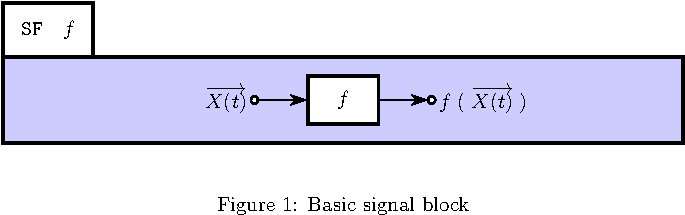
\includegraphics{figures/BasicSignalBlock}
\caption{\label{Fig:SignalBlock}Basic signal block}
\end{figure}

In the algebraic approach to constructing block diagrams, a set of
special combination operators (or combinators) are used to construct
complex signal blocks from primitive ones. We assume there is a set of
primitive blocks defined elsewhere that corresponds to arithmetic
operators and other essential functionality of the continuous
subsystem.

A model description in our notation will consist of the
combination of a number of signal blocks into a composite signal block
that specifies mathematical rules to be computed within a simulation
environment.

\subsubsection{Basic signal function combinators}
\begin{enumerate}

\item $\texttt{IDENTITY}$ represents the identity signal function; the
  input value is passed unchanged to the output.

\item $\texttt{SEQUENCE}$ is the combinator to sequentially compose
  signal functions: \[\texttt{SEQUENCE}\quad{}f_{1}\quad{}f_{2}\]

The sequential composition of $f_{1}$ and $f_{2}$ is obtained by
connecting the outputs of $f_{1}$ to the inputs of $f_{2}$.




\begin{figure}
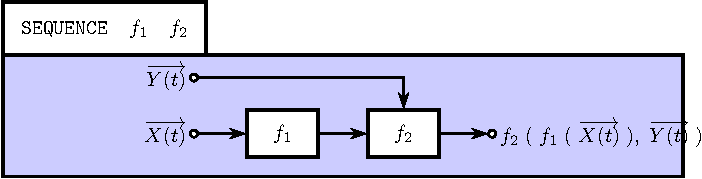
\includegraphics{figures/SequenceSignalBlock}
\caption{\label{Fig:SequenceSignalBlock}Sequence signal block}
\end{figure}

\item $\texttt{UNION}$ is the combinator to compose
  signal functions in parallel: \[\texttt{UNION}\quad{}f_{1}\quad{}f_{2}\]

The parallel composition of $f_{1}$ and $f_{2}$ is obtained by
obtaining the union of outputs of $f_{1}$ and $f_{2}$.



\begin{figure}
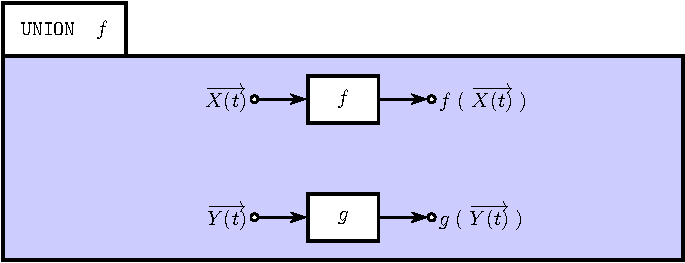
\includegraphics{figures/UnionSignalBlock}
\caption{\label{Fig:UnionSignalBlock}Union signal block}
\end{figure}

\item $\texttt{SENSE}$ selects a signal from the environment of the
  continuous subsystem and applies the given signal function to that
  signal:

\[\texttt{SENSE}\quad{}signal\quad{}f\]

\begin{figure}
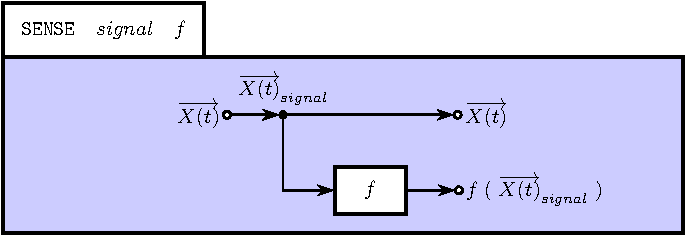
\includegraphics{figures/SenseSignalBlock}
\caption{\label{Fig:SenseSignalBlock}Sense signal block}
\end{figure}

\item $\texttt{ACTUATE}$ creates a new signal in the environment from
  the output of the given signal function:

\[\texttt{ACTUATE}\quad{}signal\quad{}f\]

\begin{figure}
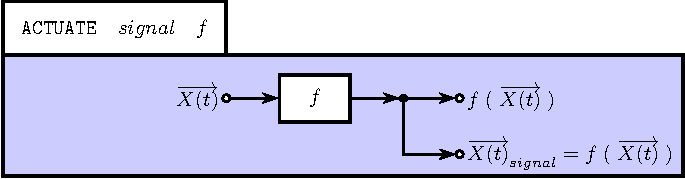
\includegraphics{figures/ActuateSignalBlock}
\caption{\label{Fig:ActuateSignalBlock}Actuate signal block}
\end{figure}

\end{enumerate}

\subsubsection{Discrete events}

An event originating in the discrete subsystem occurs at a single
point in time, and has no duration, e.g. a signal exceeding some
threshold. Events are modeled in the continuous subsystem as signals
that are only defined at the points in time when the events occur.

An event can be turned into a continuous signal by the $\texttt{HOLD}$
signal function combinator, which remembers the most recent value of
an event:

\[\texttt{HOLD}\quad{}S_{e}\quad{}::=\quad{}S_{e}(t_{i})\quad{}where \quad{}t_{i}\leqq{}t\quad{} and \quad{}\nexists{S_{e}(t_{j})}:\:t_{i}\leqq{}t_{j}\]

A continuous signal can turned into an event by the $\texttt{EDGE}$
signal function combinator, which receives a signal and generates an
event when the signal changes.

Simultaneously occurring events can be merged by the $\texttt{MERGE}$
combinator, which combines events using functions defined in the
discrete subsystem:

\[\texttt{MERGE}\quad{}I_{proc}\quad{}::=\quad{}\texttt{sf}(I_{proc}(x\;,\:\;y))\quad{}where \quad{}\langle{}x\;,\;\;y\rangle{}\in{}S_{e}(t_{i})\]


This combinator yields a merged event stream containing the events
returned by the supplied function.

\subsubsection{Transitions and Transients}

The switching primitives of the language can be used when there is a
succession of signal functions to switch into as a succession of
particular events occurs, similar to state changes in a finite state
automaton.

Suppose that the system of equations that govern the continuous
dynamics is given by a function

$F\;{\mathrm\mathbf{}(}y\;,\;\;y^{(1)}\;,\;\;\ldots\;,\;\;y^{(n-1)}\;,\;\;t{\mathrm\mathbf{})}\quad{}=\quad{}y^{(n)}$.

To represent the changes in the continuous dynamics, we will introduce
the function $G$ such
that \[G\;{\mathrm\mathbf{}(}k{\mathrm\mathbf{})}\mapsto{}F_{k}{\mathrm\mathbf{}(}y\;,\;\;t{\mathrm\mathbf{})}\]
where $k$ is a vector of boolean values that reflects the possible
modes of the continuous system. The signal function primitives then
allow the construction of all $F_{k}$. The $\texttt{TRANSITION}$ primitive
specifies when switching from one $F_{k}$ to another occurs. The
relation consisting of all $\texttt{TRANSITION}$ statements describes
function $G$.

\[\texttt{TRANSITION}\quad{}I_{event}\quad{}S_{f}\quad{}S_{fk}\]
\\

behaves as follows: $S_{f}$ is applied to the input signal and the
signal $I_{event}$ is obtained. The output signal is $S_{f}$ until an
event occurs. In that case, the output signal becomes $S_{fk}$, which
replaces $S_{f}$.


\section{\label{ap_examples}NineML Abstraction Layer Examples}

\subsection{XML}

Here are some examples of XML serialization


\subsection{Python}

Here are some examples of Python lib9ml syntax


\subsection{Native Syntax}

Here are some examples of NineML native syntax (Chicken Scheme implementation)


%\bibliography{refs}

\end{document}
